\documentclass{beamer}
\usepackage[latin1]{inputenc}
\usepackage{textpos}

\usepackage{graphics}
% \usepackage[demo]{graphicx}
\usepackage{adjustbox}

\usepackage[english]{babel}
\usepackage{colortbl}
\usepackage{caption}
% \usepackage{subcaption}
\usepackage{multirow}
\usepackage{amsmath}
\usepackage[makeroom]{cancel}
\usepackage{xcolor} % for colored text

\usepackage{tikz} % for flow charts
\usetikzlibrary{shapes,arrows,positioning,shadows,calc}

\usepackage{filecontents}% http://ctan.org/pkg/filecontents
\usepackage{silence}% http://ctan.org/pkg/silence
\WarningFilter{latex}{Overwriting file}% Remove LaTeX warnings starting with "Overwriting file"
\begin{filecontents*}{linereg.data}
#x y
0 4
10 24
\end{filecontents*} 

\begin{filecontents*}{linereg2.data}
#x y
2 8
8 20
\end{filecontents*} 

	\renewcommand<>{\item}[1]{\only#2{\beameroriginal{\item}{#1}}} % for replace a equation for other equation in the same place
	
	% \usetheme{Warsaw}
	\usetheme{Frankfurt}
	% \usetheme{Boadilla}
	\setbeamertemplate{navigation symbols}{} 
	% \useoutertheme{infolines} 
% \setbeamertemplate{footline}{\hbox{\vspace{0.1cm} \insertshortauthor \hspace*{3.5cm} \insertshorttitle \hspace*{4.0cm} \hfill\insertframenumber/\inserttotalframenumber}} 

\setbeamertemplate{footline}{\hbox{\vspace{0.1cm} \insertshortauthor \hspace*{3.5cm} \insertshorttitle \hspace*{4.4cm} \hfill\insertframenumber}} 

\def\braces#1{[#1]} % to define square parenthesis 
	
% \usecolortheme{orchid}

% \usecolortheme{lily}

% \usecolortheme{default}
\usecolortheme{cranejavier}

% \setbeamertemplate{footline}[frame number]
% \setbeamertemplate{footline}[page number]
	
	
	% -------------------------------------- Slide 1
	\title[Field Measurements and Instrumentation]{Intro to Instrumentation and Field Measurements in Remote Sensing}
	\author[Javier Concha]{\Large Javier Concha and Paul Romanczyk}
	\institute{\footnotesize Digital Imaging and Remote Sensing Lab\\Chester F. Carlson Center for Imaging Science\\ Rochester Institute of Technology}
	\date{\today}


\AtBeginSection[ ]
{	\setbeamertemplate{footline}{} 	
	\begin{frame}{\LARGE Outline} 
	\LARGE
		\tableofcontents[currentsection]
	\end{frame}

\addtocounter{framenumber}{-1}	

\setbeamertemplate{footline}{\hbox{\vspace{0.1cm} \insertshortauthor \hspace*{2.5cm} \insertshorttitle \hspace*{4.4cm} \hfill\insertframenumber}} 
}	

% \AtBeginSubsection[ ]
% {		
% 	\begin{frame}{\LARGE Outline} 
% 		\tableofcontents[currentsection,currentsubsection]
% 	\end{frame}
% \addtocounter{framenumber}{-1}	
% }		
\newcounter{tmpc} % for resume counter
%&&&&&&&&&&&&&&&&&&&&&&&&&&&&&&&&&&&&&&&&&&&&&&&&&&&&&&&&&&&&&&&
%&&&&&&&&&&&&&&&&&&&&&&&&&&&&&&&&&&&&&&&&&&&&&&&&&&&&&&&&&&&&&&&
\begin{document}
{	
\setbeamertemplate{footline}{} 
\setbeamertemplate{headline}{}
	
	\begin{frame} 
	\titlepage
	
	\begin{textblock*}{10cm}(10.0cm,-8.2cm)
	   
\includegraphics[height=10mm]{/Users/javier/Desktop/Javier/MASTER_RIT/2011_THESIS/LaTeX/Presentation/tiger_walking_rit_color.eps}
	\end{textblock*}
	
	\begin{textblock*}{10cm}(-.7cm,-8.2cm)
	   
\includegraphics[height=10mm]{/Users/javier/Desktop/Javier/PHD_RIT/ConferencesAndApplications/2014_ASPRS_SOY/Images/dirs_logo.png}
	\end{textblock*}
	
	\begin{textblock*}{9cm}(2cm,-4.5cm)

	   \tikz\node[opacity=0.3]{ 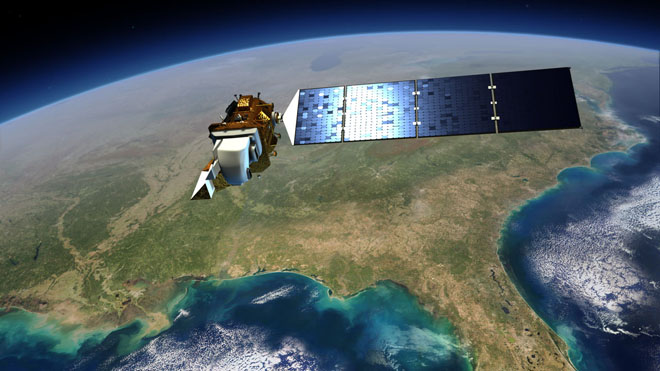
\includegraphics[width=65mm]{/Users/javier/Desktop/Javier/PHD_RIT/ConferencesAndApplications/2014_ASPRS_SOY/Images/landsat8-earth.jpg}};
	\end{textblock*}

	\begin{textblock*}{12cm}(3.0cm,0cm)
	   \scriptsize Presented for 2015 Intersession Term
	\end{textblock*}
	
	\end{frame}

}
\addtocounter{framenumber}{-1}
%\setbeamercovered{highly dynamic}
%\setbeamercovered{transparent}
\setbeamercovered{still covered={\opaqueness<1->{2}},again covered={\opaqueness<1->{2}}}

% ----------------------------------- Slide ----------------------------------------------	

\addtobeamertemplate{frametitle}{}{%
\begin{textblock*}{90mm}(8.2cm,-0.5cm)
% \includegraphics[height=0.5cm]{/Users/javier/Desktop/Javier/MASTER_RIT/SPIE2012/Slides/rit_white_no_bar.jpg}

\includegraphics[height=0.4cm]{/Users/javier/Desktop/Javier/PHD_RIT/ConferencesAndApplications/2014_ASPRS_SOY/Images/RIT_LOGO.png}
\end{textblock*}}


% ----------------------------------- Slide ----------------------------------------------
{
\setbeamertemplate{footline}{} 
\begin{frame}{\LARGE Outline} 
\LARGE
	\tableofcontents
\end{frame}

\addtocounter{framenumber}{-1}
}

%%%%%%%%%%%%%%%%%%% SECTION %%%%%%%%%%%%%%%%%%%%%%%%%%%%%%%%
\section{Introduction}
\subsection*{Motivation}
% --- slide ------------------------------------------------
\begin{frame}{\LARGE Definitions} 
\LARGE
{\bf Field Measurements or Groundtruth:}\\
\vspace{.1cm}
``Observations or measurements made at or near the surface of the earth in support of remote sensing.''\\
\vspace{.5cm}
{\bf Remote Sensing:}\\
``Remote sensing is the science of obtaining information about objects or areas from a distance, typically from aircraft or satellites.''\\

\end{frame}
% --- slide ------------------------------------------------
\begin{frame}{\LARGE Motivation} 
\large
\begin{itemize}\itemsep.3cm
\item {\bf Why is it important?}\\
\end{itemize}
\end{frame}
% --- slide ------------------------------------------------
\begin{frame}{\LARGE Motivation (con't)} 
\vspace{-.7cm}

\end{frame}
% --- slide ------------------------------------------------
\begin{frame}{\LARGE Motivation (con't)} 
\huge
{\bf PROBLEM}:\\
\vspace{.1cm}

\end{frame}
% --- slide ------------------------------------------------
\begin{frame}{\LARGE Goal} 
\end{frame}
% --- slide ------------------------------------------------
\begin{frame}{\LARGE Retrieval Process} 

\begin{figure}[H]
		\includegraphics[height=7cm]{/Users/javier/Desktop/Javier/PHD_RIT/ConferencesAndApplications/2014_ASPRS_SOY/Images/RetProcess.pdf}
\end{figure}

\end{frame}
% --- slide ------------------------------------------------
\begin{frame}{\LARGE Objectives}
\begin{itemize}
\Large
\item Develop over-water atmospheric correction
\vspace{.4cm}
\item Design water constituent retrieval algorithm
\vspace{.4cm}
\item Apply glint correction
\vspace{.4cm}
\item Validate results
\vspace{.4cm}
\item Demo process to a different study site
\end{itemize}
\end{frame}
%%%%%%%%%%%%%%%%%%% SECTION %%%%%%%%%%%%%%%%%%%%%%%%%%%%%%%%

%%%%%%%%%%%%%%%%%%% SECTION %%%%%%%%%%%%%%%%%%%%%%%%%%%%%%%%
\section{Conclusions}
\subsection*{Conclusions}
% --- slide ------------------------------------------------
\begin{frame}{\LARGE Conclusions}

\Large
\begin{itemize}\itemsep.4cm
	\item Current retrieval algorithm depends on IOPs from the field. Not always available!

	\item LUT from Hydrolight: Highly dependent in phase function

	\item Obtain field data for Landsat-8 is difficult, mainly for weather conditions
\end{itemize}

\end{frame}

% --- slide ------------------------------------------------
{	
\setbeamertemplate{footline}{} 
\setbeamertemplate{headline}{}
\begin{frame}[noframenumbering] 

\vspace{\baselineskip}
\centerline{\Large Thanks for your attention!}
	\vspace{\baselineskip}
\vspace{-.3cm}
% \centerline{\Huge QUESTIONS?}
\uncover <2->{\centerline{\Huge QUESTIONS?}}
\vspace{\baselineskip}
\centerline{Javier A. Concha}
\centerline{jxc4005@rit.edu}

\begin{figure}[htb]
\centering
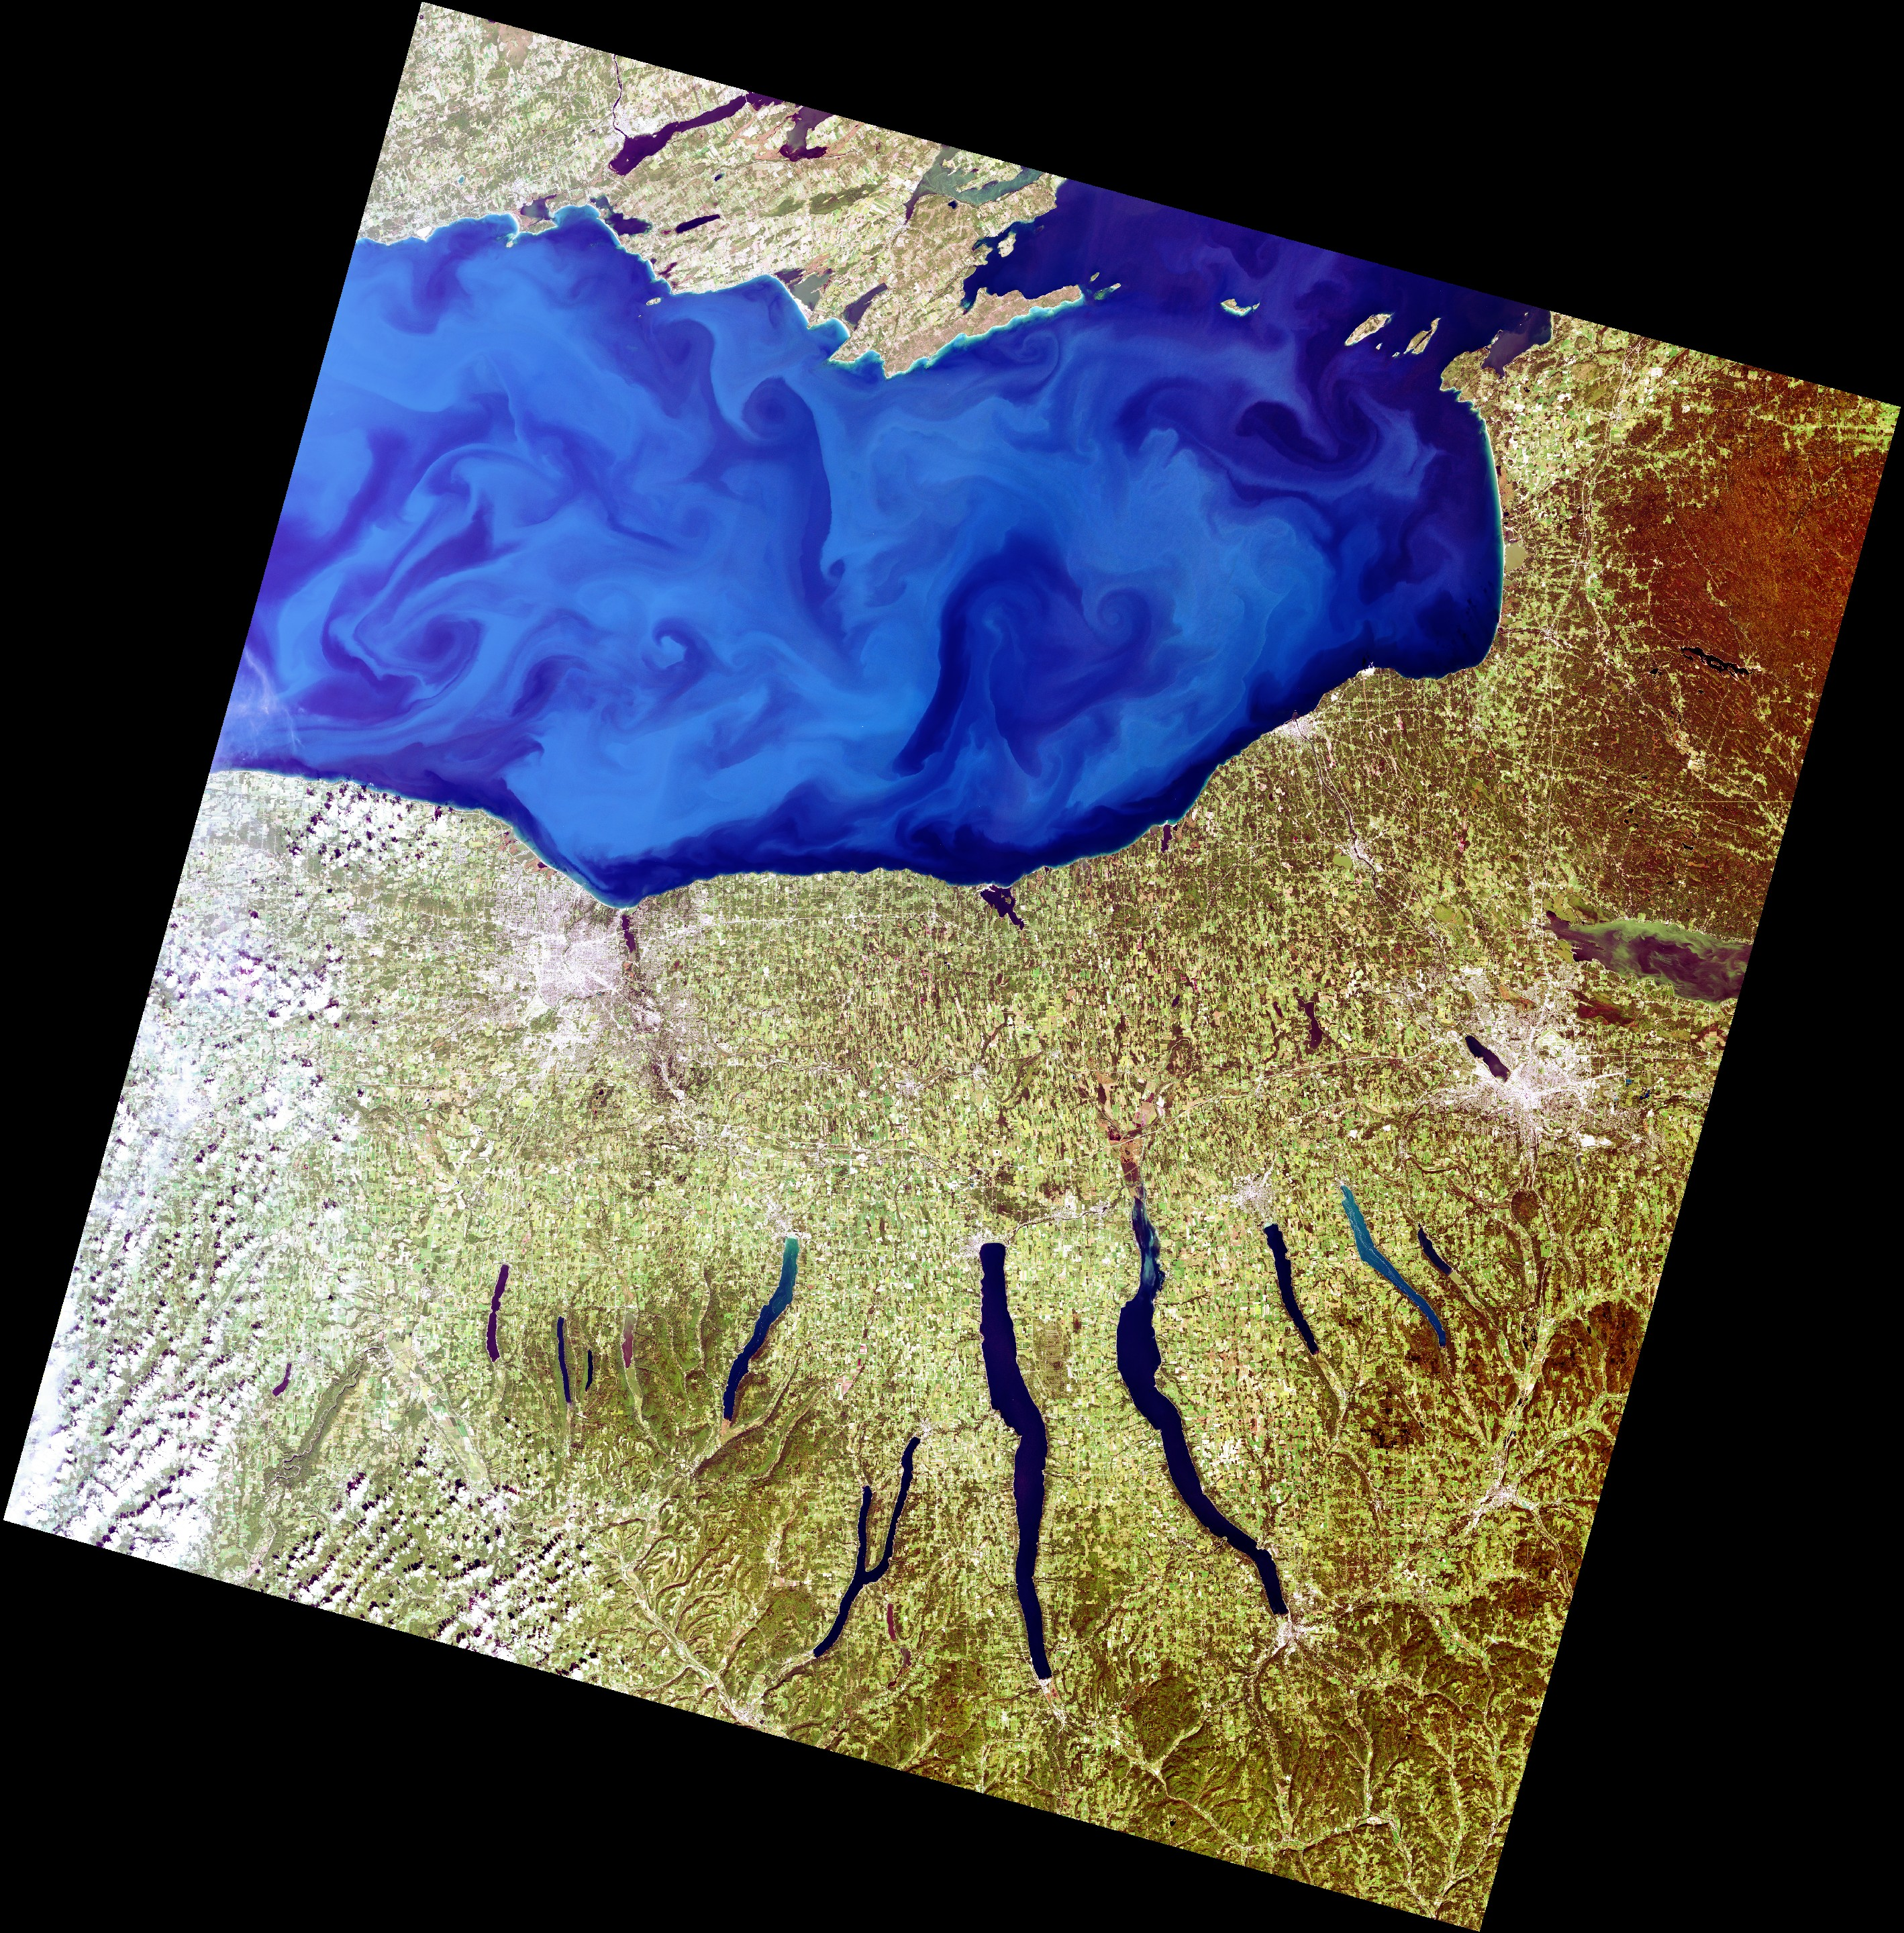
\includegraphics[height=5cm]{/Users/javier/Desktop/Javier/PHD_RIT/ConferencesAndApplications/2014_ASPRS_SOY/Images/LC80160302013262LGN00.jpg}
\end{figure}
\vspace{-.5cm}
\centerline{\tiny (09/19/2013)}
\end{frame}
}
% % BIBLIOGRAPHY
% \bibliographystyle{apalike}

% \bibliography{/Users/javier/Desktop/Javier/PHD_RIT/Latex/javier_bib}
% --- slide ------------------------------------------------
\section*{}
\begin{frame}%[shrink=30] 
\tiny
  \frametitle{References}
  % \nocite{*}
  \bibliographystyle{apalike}
  \bibliography{/Users/javier/Desktop/Javier/PHD_RIT/Latex/javier_bib}
\end{frame}
\end{document} 
% EEEEEEEEEEENNNNNNNNNNNNNNDDDDDDDDDDDD